\documentclass[11pt]{article}

\author{Math 106}
\date{Due Friday, Sept 22 by 11:59pm} 
\title{Homework 2}

\usepackage{graphicx,xypic}
\usepackage{amsthm}
\usepackage{amsmath,amssymb}
\usepackage{amsfonts}
\usepackage{xcolor}
\usepackage[margin=1in]{geometry}
\usepackage[shortlabels]{enumitem}
\newtheorem{problem}{Problem}
\renewcommand*{\proofname}{{\color{blue}Solution}}


\setlength{\parindent}{0pt}
\setlength{\parskip}{1.25ex}


\begin{document}

\maketitle

% You are required to put your name here:
{\bf\Large Name:} 


\vspace{.3in}
Topics covered: unit-speed parameterizations, curvature, bicycles

Instructions: 
\begin{itemize}
\item This assignment must be submitted on Gradescope by the due date. 
\item If you collaborate with other students (which is encouraged!), please mention this near the corresponding problems. 
\item If you are stuck, please ask for help (from me, a TA, a classmate). Use Campuswire!  
\item You may freely use any fact proved in class. In general, you should provide proof for facts used that were not proved in class. 
\item Please restrict your solution to each problem to a single page. Usually solutions can be even shorter than that. If your solution is very long, you should think more about how to express it concisely.
\end{itemize}
\pagebreak 



\begin{problem}
Give a unit-speed parameterization of the logarithmic spiral.
\end{problem}

\begin{proof}

\end{proof}

\pagebreak

\begin{problem}
In this problem you work out a formula for curvature of a space curve that's not necessarily unit speed. Let $\beta:[a,b]\to\mathbb R^3$ be a curve (not necessarily unit speed!), and let $g(t)=\int_a^t|\beta'(u)|\>du$ be its arclength function (in particular $g'(t)=|\beta'(t)|$). From class, we can define a unit speed curve $\alpha$ so that $\alpha\circ g=\beta$. The curvature $\kappa(t)$ of $\beta$ at time $t$, is by definition the curvature of $\alpha$ at time $g(t)$, which we will define in class as $|\alpha''(g(t))|$.  
\begin{enumerate}[(a)]
\item Derive from this setup that the curvature of $\beta$ is give by the formula
\[\kappa(t)=\frac{|T'(t)|}{g'(t)},\]
where $T(t)$ is defined as $\beta'(t)/|\beta'(t)|= \beta'(t)/g'(t)$. \footnote{Hint: apply the first rule of differential geometry (twice). }
\item Derive the formula 
\[\kappa(t)=\frac{\beta'(t)\times\beta''(t)}{|\beta'(t)|^3}
\]\footnote{Hint: first differentiate $\beta'=g'T$ to get a formula for $\beta''$.}
\end{enumerate} 
\end{problem}

\begin{proof}

\end{proof}

\pagebreak

\begin{problem}[B, 1.3.4]
Let $f:I\to\mathbb R$ be a smooth function, and define $\alpha(t)=(t,f(t))$ (the trace of $\alpha$ is the graph of $f$). Compute the curvature of $\alpha$. \footnote{Hint: Your solution should be painless. } 
\end{problem}

\begin{proof}

\end{proof}

\pagebreak

\begin{problem}
Consider a bike traveling in the plane. Let $\alpha(t)$ and $\beta(t)$ be the positions of the front and back wheels at time $t$, respectively.\footnote{More precisely, think of the position that each wheel touches the ground.} Assume $\alpha$ is unit speed and that the distance between the wheels is one unit. If $\alpha$ is known, how do we determine $\beta$? (That's what you'll figure out here.) 

\begin{enumerate}[(i)]
\item Since $\alpha'(t)$ and $N(t)$ are an orthonormal basis for each $t$, we can write 
\[\alpha-\beta=(\cos\theta) \alpha'+(\sin\theta) N\] for some function $\theta$. \footnote{Physically, $\theta(t)$ is the angle that the front wheel is turned at time $t$.} Use this to express $\beta'$ as a linear combination of $\alpha'$ and $N$. \footnote{The coefficients will involve $\theta$ and the curvature $\kappa$ of $\alpha$.} 

\item Since the rear wheel always points in the direction $\alpha-\beta$, we also know $\beta'=\lambda(\alpha-\beta)$ for some function $\lambda$. Compute $\lambda$. \footnote{Observe that $\lambda=\beta'\cdot(\alpha-\beta)$.}

\item Combine the previous two parts to write a differential equation\footnote{``Differential equation" just means an equation satisfied by functions that also involves their derivatives.} satisfied by $\theta$ and $\kappa$. \footnote{This differential equation can be used to simplify the equation for $\beta'$ in part (i).}
\end{enumerate} 
\end{problem}

\begin{proof}

\end{proof}

\pagebreak


\begin{problem}
Below is the tire tracks of a bike. 
\begin{center}
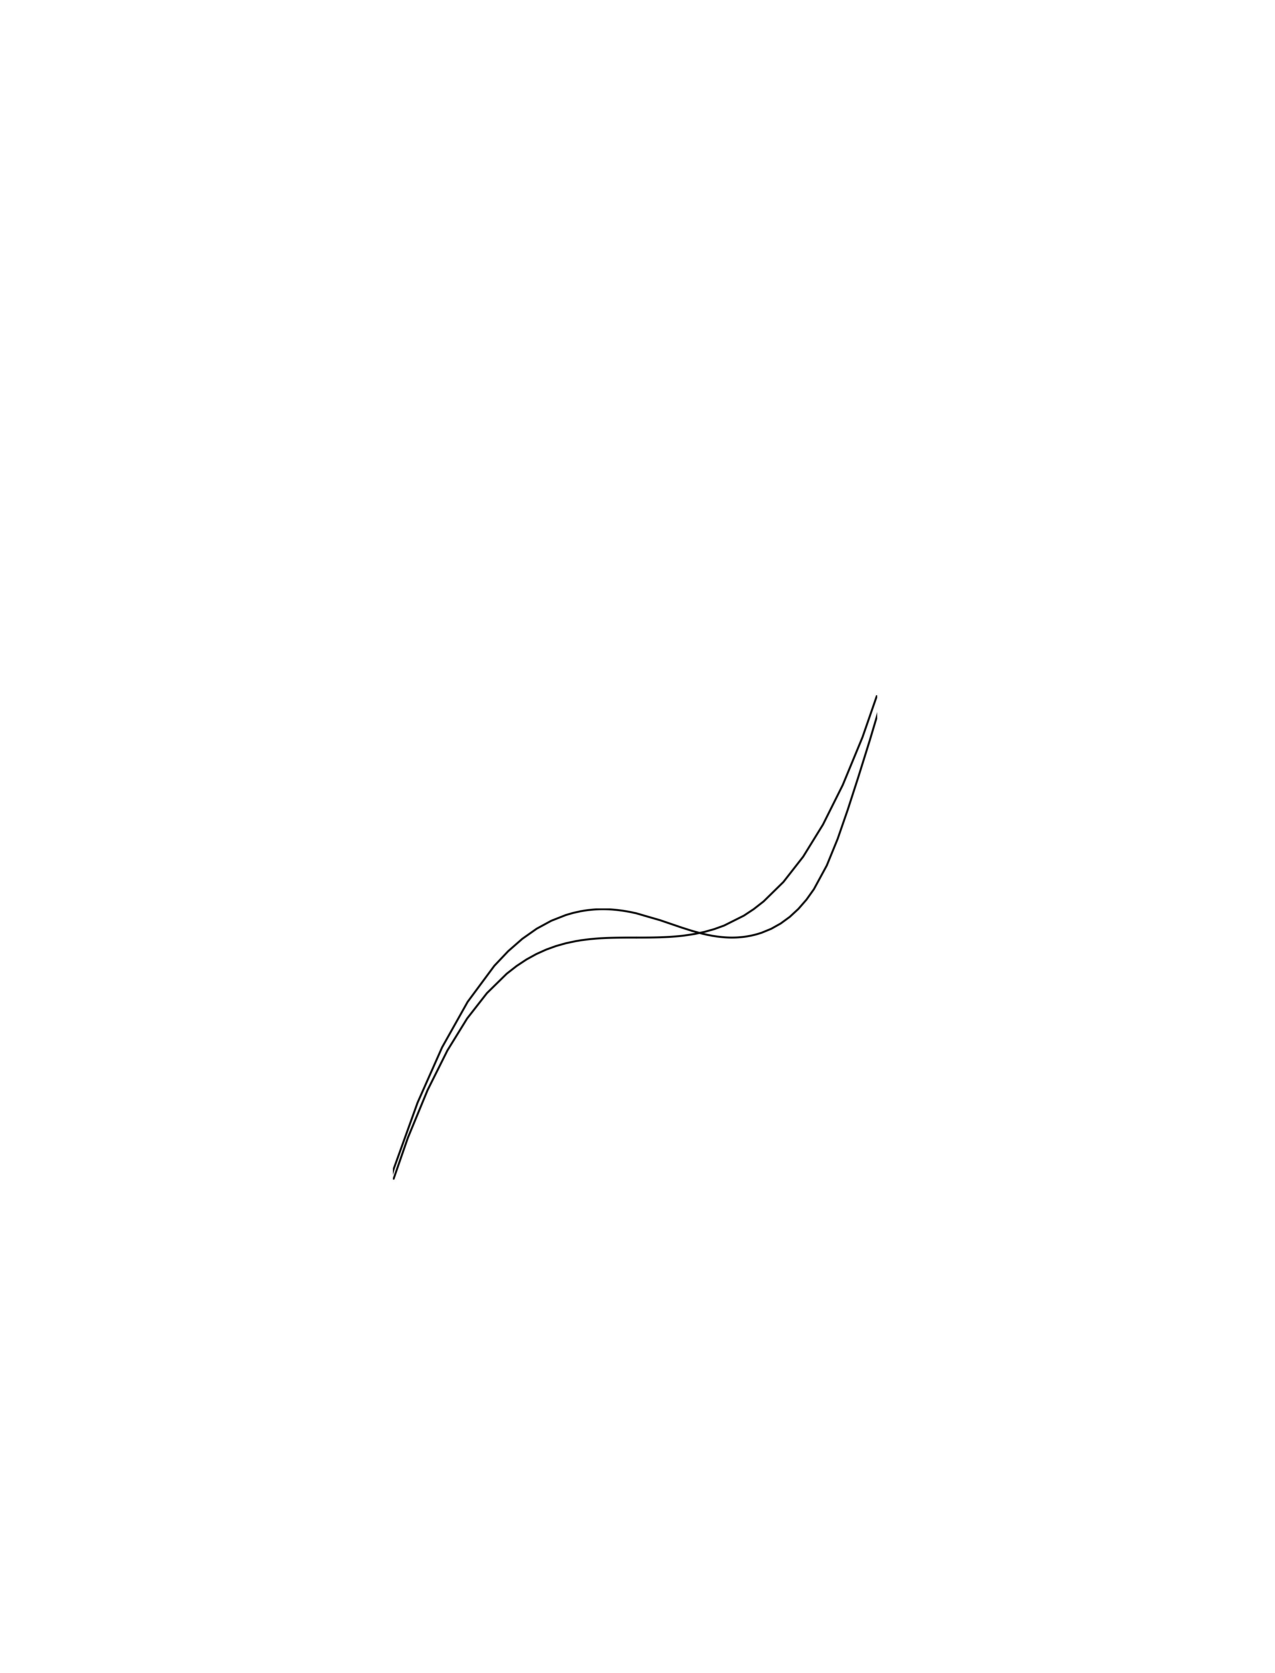
\includegraphics{bike.pdf}
\end{center}
Which is the front/back wheel? Which direction was the bike traveling? \footnote{Hint: The tangent line through one of the curves always intersects the other curve...}
\end{problem}

\begin{proof}

\end{proof}




\end{document}